\section{Results}
\label{sec:results}

Determining the value for the threshold current requires careful adjustment of the unattenuated laser power. For the LED regime,
in which spontaneous emission dominates the light production, stable interference patterns cannot exist. This means that the
light on the IR viewing card appears diffuse and symmetrical. As soon as stimulated emission begins to dominate, the diode
operates in the LASER regime. The now coherent wave interacts with the texture of the card surface and creates a stable asymmetrical
image. The observed type of diffraction occurs due to the various bumps and grooves roughly matching the wavelength in size, resulting
in random granulation as predicted by Huygens principle. 

\begin{figure}
    \begin{subfigure}{0.48\textwidth}
        \centering
        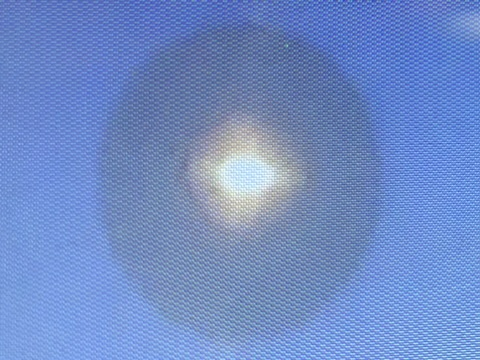
\includegraphics[width=\linewidth]{content/measurement/led.jpg}
        \caption{LED regime at $I = \qty{34.4}{\milli\ampere}$.}
        \label{fig:pattern_led}
    \end{subfigure}
    \hfill
    \begin{subfigure}{0.48\textwidth}
        \centering
        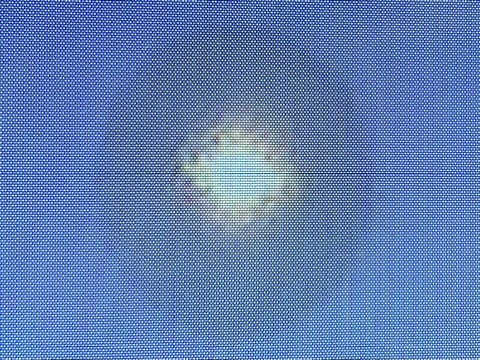
\includegraphics[width=\linewidth]{content/measurement/laser.jpg}
        \caption{LASER regime at $I = \qty{34.6}{\milli\ampere}$.}
        \label{fig:pattern_laser}
    \end{subfigure}
    \caption{Comparison of light pattern slightly below and above the chosen threshold current $I = \qty{34.5}{\milli\ampere}$.
             Notice the diffuse reflection on the left versus the coarse granulation on the right. These distinct appearances
             are the results from random diffraction of incoherent or coherent waves respectively.}
    \label{fig:pattern}
\end{figure}

The described patterns slightly below and above the current threshold can be viewed in Figure \ref{fig:pattern}. For the given
apparatus, visual examination yields $I = \qty{34.5}{\milli\ampere}$ for the minimum lasing value, though there is some ambiguity,
as will be discussed later.

\begin{figure}
    \centering
    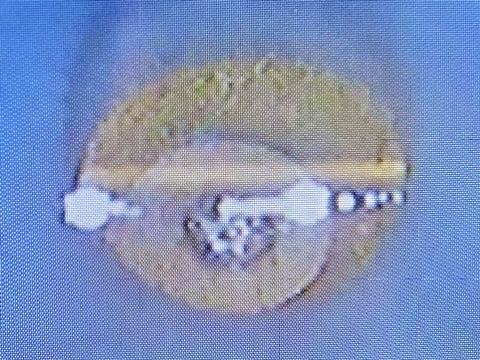
\includegraphics[width=0.48\linewidth]{content/measurement/fluorescence.jpg}
    \captionsetup{width=0.58\linewidth}
    \caption{Rubidium flourescence line along the laser beam as seen through the observation window in the vapor cell.}
    \label{fig:fluorescence}
\end{figure}

\begin{figure}
    \centering
    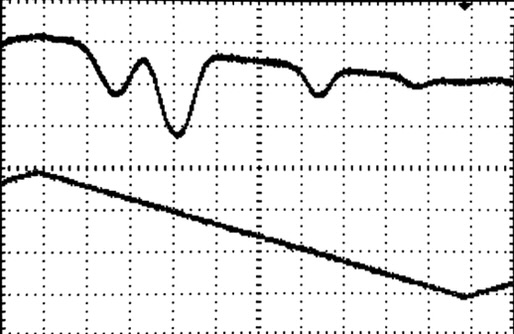
\includegraphics[width=0.72\linewidth]{content/measurement/ramp.jpg}
    \captionsetup{width=0.8\linewidth}
    \caption{Modulated signal without correction (top). Triggered ramp output for laser and piezo stack (bottom).
             As previously described, the expected linear proportionality between the two currents is clearly visible
             outside the absorption dips.}
    \label{fig:ramp}
\end{figure}

\begin{figure}
    \centering
    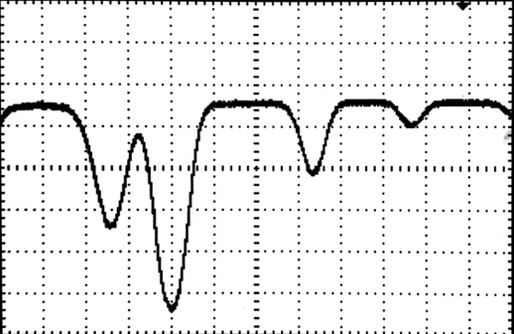
\includegraphics[width=0.72\linewidth]{content/measurement/spectrum.jpg}
    \captionsetup{width=0.8\linewidth}
    \caption{Spectrum after manual compensation via background subtraction for the scanning current contribution.}
    \label{fig:spectrum}
\end{figure}
